
The purpose of this chapter is to give an overview of the research areas
involved in this dissertation. First we explain the fundamental ideas of logic
programming and Prolog; next, tabling by call variance is described, focusing on
the execution strategy and data structures; finally, tabling by call subsumption
and related strategies like \textit{time stamped tries} are explained.

\section{Logic Programming}

Logic programming presents a declarative style of programming based on mathematical
logic and the predicate calculus. It is a very high level programming
paradigm that allows the programmer to focus on the problem at hand, leaving the
steps on \textit{how} to solve the problem to the computer.

In its purest form, logic programming is solely based on Horn Clause Logic \cite{Lloyd-87},
a subset of First Order Logic. Programming in logic can be viewed as
a two step process: (1) first, the theory is formulated as logic clauses,
next (2) we use this theory to search for alternative ways in which an arbitrary query is satisfied.

Logic programming is often mentioned to include the following advantages \cite{Carlsson-PhD}:

\begin{itemize}
  \item \textbf{Simple declarative semantics}: a logic program is simply a collection of predicate logic clauses.
  \item \textbf{Simple procedural semantics}: a logic program can be read as a collection of recursive procedures. In Prolog, for instance, clauses are tried in the order they are written and goals within a clause are executed from left to right.
  \item \textbf{High expressive power}: Logic programs can be seen as executable specifications that despite their simple procedural semantics allow for designing complex and efficient algorithms.
  \item \textbf{Inherent non-determinism}. Since in general several clauses can match a goal, problems involving search are easily programmed in these kind of languages.
\end{itemize}

\subsection{Logic Programs}

A logic program is composed by a set of Horn clauses. Each clause is a disjunction of literals
and contains at most one positive literal. Horn clauses are usually written as

\begin{center}
  $L_{1}, ..., L_{n} \Longrightarrow L  (\equiv \neg L_{1} \vee ... \neg L_{n} \vee \neg L)$
\end{center}

or

\begin{center}
  $L_{1}, ..., L_{n}  (\equiv \neg L_{1} \vee ... \neg L_{n})$
\end{center}

where $n >= 0$ and $L$ is the only positive literal. 

A Horn clause that has exactly one positive literal is called definitive clause; in the Prolog language
it is usually called a \textit{rule}.
A Horn clause without a positive literal is called a \textit{goal}.

Using Prolog's notation, one can write \textit{rules} in the form

\begin{center}
  $L :- L_{1}, ..., L{n}.$
\end{center}

Usually, $A$ is called the \textit{head} of the \textit{rule} and $L_{1}, ..., L_{n}$
the \textit{body} of the \textit{rule}, where each $L_{i}$ is called a subgoal.
A logical \textit{fact} is a special \textit{rule} where the \textit{body} is replaced by \textit{true} symbol:

\begin{center}
  $L.$
\end{center}

Goals are \textit{rules} without the \textit{head} component and are also named as \textit{queries}.


Each literal in Horn clause has the form $p(t_{1}, ..., t_{n})$, where $p$ is the \textit{predicate} symbol or \textit{functor}
and each $t_{i}$ are \textit{terms}. A term can be a \textit{constant} (or \textit{atom}), a \textit{variable}
or a \textit{compound} term. Compound terms follow the predicate structure, recursively.
Variables are assumed to be universally quantified and have the following major characteristics:

\begin{itemize}
  \item Variables are logical variables that can instantiated only once.
  \item Variables are untyped until instantiated.
  \item Variables are instantiated via \textit{unification}, a pattern matching operation that finds the most general common instance of two data objects. 
\end{itemize}

A sequence of clauses with the same functor in the head form a \textit{predicate}. The ordering
of these clauses can have some implications depending on the resolution semantics of the underlying language.
Prolog for instance, uses a top-down resolution mechanism known as \textit{SLD} (Selective Linear Definite) resolution \cite{Lloyd-87}.

SLD starts by matching the first subgoal query to the first clause of the respective predicate,
generating a new query using the body of the clause, which is added to the remaining query subgoals.
During this process a finite set of pairs $\theta$ called \textit{substitution} is built.
Each pair has the form $X = t$, where $X$ is a variable and $t$ is a term. No variable in the left-hand side
of a pair appears on the right-hand side and no two pairs have the same variable as left-hand side \cite{Sterling-94}. 
When the clause body is reused as query, all the variables present in the terms are replaced using the
set $\theta$. 

If unification fails, the next clause of the predicate is tried, in a mechanism called \textit{backtracking}.
This recursive computation fails when there are any more clauses left to try. It succeeds when the subgoal query is empty.

The resolution process is fundamentally non-deterministic and can be viewed as a search within a tree. SLD
does not force any specific search strategy for exploring the tree. Prolog for example, uses a depth-first, one
branch at a time search.

\subsection{Prolog and WAM}
  
Prolog is one of the first logic programming languages and arguably the most successful.
The first implementation of Prolog was Marseille Prolog, developed in 1972 by Alain Colmerauer and Robert Kowalski \cite{Kowalski-74}.

The use of Prolog as a practical and efficient language was made viable by David Warren in 1977, when he built a compiler that could
compete with other languages like Lisp \cite{Warren-77}. Then in 1983, David Warren formulated an abstract machine known as WAM
(\textit{Warren Abstract Machine}) \cite{Warren-83} that is still widely used in modern Prolog implementations.

\subsubsection{Prolog}

Prolog follows the semantics of the SLD resolution through a depth first search strategy.
It starts by choosing the top-most clauses of the predicate and the subgoals are solved
within a left-to-right fashion.

For illustration purposes, we defined the factorial predicate (Listing \ref{factorial_prolog}) that can compute the factorial of
any given number. This predicate has arity of 2, where the first argument is an \textit{input} argument and the second argument
an \textit{output} argument.

\begin{lstlisting}[language=prolog,basicstyle=\footnotesize,float,frame=single,caption={Factorial function in Prolog.},label=factorial_prolog]
factorial(0, 1) :- !.
factorial(N, R) :-
  N > 0,
  N1 is N - 1,
  factorial(N1, R1),
  R is R1 * N.
\end{lstlisting}

Factorial is composed of two clauses, one represents the factorial base case (factorial of 0 is 1) and
the other represents the recursive relation. The second clause first checks if the input number
is positive, to discard non-positive numbers, then computes $N - 1$ and recursively
calls factorial to compute the value of $factorial(N-1)$, finally, the variable $R$ is then unified
to $N * factorial(N-1)$. The first clause uses the \textit{cut} operator that tells the Prolog engine to not explore alternative
clauses, i.e., the factorial of 0 is not to be computed with the recursive relation declared on the second clause.

\begin{figure}[ht]
  \centering
    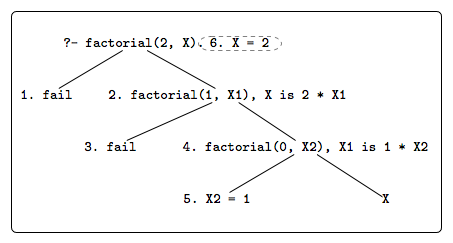
\includegraphics[scale=0.6]{factorial.png}
  \caption{Factorial search tree.}
  \label{fig:factorial_tree}
\end{figure}

Once Prolog finds the first solution (Figure \ref{fig:factorial_tree}), the cut control operator disables further
alternatives, completing the depth first search in the tree.

The cut operator is not the only special instruction in Prolog, more built-in predicates are also available:

\begin{itemize}
  \item \textbf{Meta-logical predicates}: inquire the state of the computation and manipulate terms.
  \item \textbf{Extra-logical predicates}: they can manipulate the Prolog database, adding or removing clauses from
  the program being executed. Input/Output operators are another example of extra-logical predicates.
  \item \textbf{Other predicates}: predicates to perform arithmetic operations, to compare terms, to support debugging, etc.
\end{itemize}

These special operators make programming more practical and useful in real world applications.

\subsubsection{WAM}

The WAM is an abstract machine based on a stack-based architecture with various data areas, registers, and low level instructions
that can be efficiently executed, manipulated and optimized.

The WAM uses the following execution stacks:

\begin{itemize}
  \item \textbf{Code Area}: Contains the compiled instructions.
  \item \textbf{PDL}: A push down list used by the unification process.
  \item \textbf{Trail}: Stores the addresses of the variables that must be reset when backtracking.
  \item \textbf{Stack}: Stores \textit{environment} and \textit{choice point} frames. Environments track the flow control in a program
  and choice points store open alternatives, which are used to restore the state of the computation when backtracking.
  \item \textbf{Heap}: Array of data cells used to store variables and compound terms that cannot
  be stored in the stack.
\end{itemize}

For the registers, WAM defines the following:

\begin{itemize}
  \item \textbf{S}: used during the unification of compound terms.
  \item \textbf{HB}: it is set to contain the value of the register \textbf{H} at the time of latest choice point. This is used to
  determine \textit{conditional} variable bindings that affect variables existing before the creation of the choice point.
  \item \textbf{P}: points to current WAM instruction.
  \item \textbf{CP}: stores the value of \textbf{P} before the current invoked call and it is used to restore the execution point.
  \item \textbf{TR}: points to the top of the trail stack.
  \item \textbf{E}: points to the current active environment.
  \item \textbf{B}: the active choice point.
  \item \textbf{H}: points to the top of the heap stack.
\end{itemize}

WAM instructions can be grouped into four main groups: choice point instructions to manipulate choice points; control
instructions to manage environments and control the execution flow; unification instructions that implement
specialized versions of the unification algorithm; and indexing instructions to efficiently determine which clauses
unify with a given subgoal call.

The WAM being a complex topic has complete books dedicated in explaining its intricacies.
An example is the \textit{Warren's Abstract Machine -- A Tutorial Reconstruction} written by H. A\"{\i}t-Kaci \cite{Aitkaci-91}. 

\section{Tabling}
  \subsection{Yap and XSB}
  
  \subsection{Table Space}
    \subsubsection{Tries}
    \subsubsection{Subgoal frames}
    \subsubsection{Choice Point and Execution}
  \subsection{Tabling by call subsumption}

